\section{Discussion} \label{sec:discussion}

\begin{itemize}

    \item

        Discuss that we would have liked to train an RNN on the character limit
        but that we did not have the computation power.

    \item

        Discuss how comparable our results will be with data in the real world.
        We had no texts written by actual ghost writers so we have no idea how
        our networks would perform on such texts.

    \item

        Discuss how different weight functions performed compared to other
        weight functions and describe why we think that is the case.

    \item

        Generate AUROC curves for our networks and discuss the output.

    \item

        Discuss that we beat our baselines but were not able to beat the MaCom's
        restrictions.

\end{itemize}

\subsection{Results}

Looking at the results presented in Section \ref{sec:results} it is apparent
that we have not achieved less the than 10\% accusation error on the test
set that MaCom required We believe however that some of the methods show
promising results. While all the networks we applied to the the test set beat
our baselines the best performing network was the \gls{conv-char-NN}. This
network had an accusation error closest to to the one required in addition to
having the highest overall accuracy in all the categories we tested it on.
While this network was in fact the best, it was closely followed by network
\gls{conv-char-word-NN}, while the \gls{rec-sent-NN} we also tested had sub-par
performance, lending credence to the applicability of \gls{CNN}s to \gls{NLP}
problems. It is however worth noting that this could very well be due to the
infeasibility of running any of our \gls{RNN}s on the character level of the
texts supplied to it. Looking at the performance of the two \gls{CNN}s, it
becomes obvious that the character level is of great importance when it comes
to determining the author of a text. The sentence level is simply to high of
a linguistic level. At least in the way we applied it. We hypothesize that
applying it to a lower level, such as the word level would greatly increase its
performance, as \gls{RNN}s would be able learn based on the words relation to
one another, and therefore use a more grammar based learning approach. Looking
at \gls{conv-char-NN}, and \gls{conv-char-word-NN}, it would seem that focusing
on the word level of the texts seem to actually hurt the model a bit. We are a
bit uncertain as to the reason for this, we do however have some theories. The
reason might be similar to the problem \gls{rec-sent-NN} had. The level might
actually be a bit to high for our convolutional networks, the image-equivalent
of having a to large convolutional window, thus ignoring all the small details
that are needed in order to properly determine the author. This also highlight a
potential reason behind the differing performance of networks \gls{conv-char-NN}
and \gls{conv-char-word-NN}. \gls{conv-char-NN} had many filters on the
character level of the text, whereas \gls{conv-char-word-NN} had more filters on
the word level. This might very well have led to \gls{conv-char-word-NN} missing
some relevant person-specific traits on the character level such as typos, dot
position, comma positions and the like. It wouldn't even be able to find such
traits on the word level, as the usage of a pre-trained embedding layer means
that only correctly spelled word were even considered.

Another \gls{NLP} advantage \gls{CNN}s has in this context, is the fact that
we are able to more accurately determine what part of the text contributed to
final classification as can be seen in the following section.


\subsection{Teacher Feedback}

In our introduction we reported that we wanted to look at what kind of feedback
we could give to teachers in conjunction with the bare predictions. As explained
earlier the system is not meant to be the final judge of which students are
cheating but are rather meant as a support system for teachers that are
already suspicious. We have looked at what kind of feedback we could give to
teachers. We have focused on the \gls{conv-char-NN} network since it performed
best on the test dataset. We have previously looked at the output of the
feature extraction layer to obtain information on what a specific network
were looking at. We wanted to do something similar for teacher feedback.
Recall that \gls{conv-char-NN} started with a convolutional layer followed
by a max pool layer. We therefore know that the larger the output of the
convolutional layer the more important that particular character sequence
is. The output of the feature extraction can be thought of as in Figure
\ref{fig:feature_extraction_output_example}. Each filter gives a single
output that is the maximum output in any filter position. The combining function
for the third network was the absolute difference. That means that when we
are comparing $t$ and $t'$. That means that the output of the combination
will be high for a particular filter iff the maximum output of that filter is
significantly different for $t$ and $t'$.

\begin{figure}
    \centering
    \textbf{Teacher Feedback Script Example}\par\medskip
    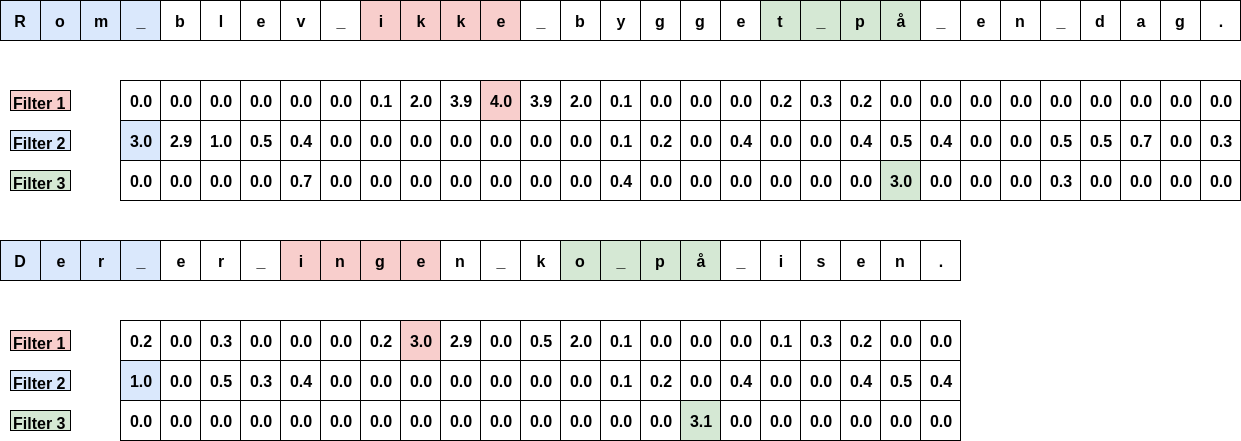
\includegraphics[width=\textwidth]{./pictures/discussion/teacher_feedback_example.png}
    \caption{Illustrates our script that gives feedback to teachers. The
        particular network used in this example only has three filters. The
        three filters maximum activations are shown in three different colors
        for the two texts they are comparing. The first filter looks for
        negative qualifiers. Therefore it reacts strongly to both the Danish
        word "ikke" (not) and the Danish word "ngen" (noone). The second filter
        looks for city names so it reacts strongly to the string "Rom " (Rome)
        but less strongly to "Der " (not a city name) even though it looks like
        a city name. The third filter reacts to phrases that contains the word
        "p\aa " (on) and therefore reacts about the same to both texts.}
    \label{fig:feature_extraction_output_example}
\end{figure}

It is hard to know exactly what the following layers does with the absolute
difference but we feel that it is a fair assumption that the largest filter
differences translates to the most important differences. The feedback system
we implemented for teachers takes an author $\alpha$, text $t$ and $n \in
\mathbb{N}^+$ and outputs the $n$ largest differences between each $t' \in
T_\alpha$ and $t$. The idea is that the when our system reports a negative the
teacher can ask for feedback from the system. The teacher will then get a list
of the $n$ greatest differences between each of the texts and can use that
information to argue against the student.

As an example we ran our system on a random author and a text that that author
did not write. The whole output of three different texts can be seen in Appendix
\ref{subsec:teacher_feedback_text_comparisons} through \ref{TODO}. We have shown
a truncated output in Table \ref{tab:teacher_feedback_output}.

\begin{table}
    \begin{tabular}{llll}
        \textbf{Filter} & \textbf{Activation Text 1} &
        \textbf{Activation Text 2} & \textbf{Difference} \\
        \hline
        426 & \verb'"; ”Hvis "'  & \verb'". Et kla"' & $|2.82 - 4.57| = 1.75$ \\
        71  & \verb'"dem; Nia"'  & \verb'"der skri"' & $|4.64 - 3.16| = 1.45$ \\
        549 & \verb'". Jeg vi"'  & \verb'". Her is"' & $|2.61 - 4.02| = 1.41$ \\
        288 & \verb'" 2 af 2\n"' & \verb'"og refle"' & $|4.90 - 3.53| = 1.37$ \\
        496 & \verb'" udseend"'  & \verb'"vad litt"' & $|2.78 - 4.12| = 1.34$ \\
        33  & \verb'"et sind."'  & \verb'"risning,"' & $|3.05 - 4.36| = 1.31$ \\
        460 & \verb'" 2 af 2\n"' & \verb'" krig og"' & $|3.69 - 2.43| = 1.26$ \\
        514 & \verb'", derfor"'  & \verb'", i forb"' & $|3.82 - 5.06| = 1.24$ \\
        531 & \verb'" om, for"'  & \verb'" om, hva"' & $|4.64 - 5.84| = 1.20$ \\
        458 & \verb'"Derudove"'  & \verb'"derfor b"' & $|4.31 - 3.13| = 1.18$ \\
        \\
        261 & \verb'".\n\n\n"'   & \verb'"– de"'     & $|1.72 - 2.70| = 0.98$ \\
        484 & \verb'"lv; "'      & \verb'" dét"'     & $|2.02 - 2.96| = 0.94$ \\
        17  & \verb'"st ”"'      & \verb'"gt; "'     & $|2.57 - 3.45| = 0.88$ \\
        145 & \verb'"ndet"'      & \verb'" Det"'     & $|2.37 - 3.25| = 0.88$ \\
        299 & \verb'"osse"'      & \verb'"– de"'     & $|3.12 - 3.98| = 0.86$ \\
        477 & \verb'"f 2\n"'     & \verb'"v og"'     & $|3.05 - 2.20| = 0.85$ \\
        421 & \verb'" 13."'      & \verb'" vel"'     & $|3.03 - 2.19| = 0.84$ \\
        434 & \verb'"am; "'      & \verb'" dét"'     & $|1.18 - 2.00| = 0.82$ \\
        27  & \verb'"n to"'      & \verb'"Dett"'     & $|2.20 - 2.99| = 0.79$ \\
        445 & \verb'" om,"'      & \verb'" – S"'     & $|2.51 - 3.27| = 0.76$ \\
    \end{tabular}
    \caption{Shows the 10 most different activations of convolutional filters on
        two different texts. Both the 10 most different activations for the
        filter of size 8 and size 4 is shown. The strings that produced the
        activation are shown and the actual activations are shown to the right.}
    \label{tab:teacher_feedback_output}
\end{table}

We also looked at whether or not we could say something about which parts of an
assignment are the most likely to be ghost written. That would allow a teacher
that is suspicious of a student to identify the part of the assignment that were
least likely to be written by him and look closely at that. To do that we wrote
a script that splits a text into paragraphs and use \gls{conv-char-NN} to get a
score for each paragraph. We can then report which of the paragraphs of the text
are the most likely to be ghost written. To test our script we chose an author
$\alpha$ from the validation dataset C with $|T_\alpha| = 19$. We also chose a
random text $t \in \overline{T_\alpha}$. We took out one of the texts $t' \in
T_\alpha$ and let $T = T_\alpha \setminus \{t'\}$. We then combined $t$ and $t'$
into $t''$ such that $t''$ consist of all of the text $t'$ followed by a random
paragraph from the text $t$. That is we constructed a text $t''$ that consisted
of a text in $T_\alpha$ followed by a single paragraph not from $T_\alpha$. We
then used our script to predict which part of $t''$ was most likely written by
a ghost writer. We would expect that the last paragraph in $t''$ would be the
most likely. The output of the script was a vector of the probabilities that
each paragraph was written by the candidate author.

\begin{equation}
    (0.66320, 0.60432, 0.54737, 0.47438, 0.30528)^T
\end{equation}

As expected the last paragraph is the least similar and therefore most likely to
be written by someone else. We are now able to give a teacher an idea of why our
network makes the predictions it does. We can give feedback on which parts of
the text is the least characteristic of an authors writing style and we can give
feedback on why the network thinks that. Of course a teacher will still have to
make the ultimate decision but can use the output of the network to underpin his
or her accusation.


\subsection{Applicability of Method}

In this section we will discuss how applicable our approach will be to real
world situations. We have created our solutions in a lab setting which
simplifies the problem quite a bit. We discuss here how our results can be
applied to find real ghost writers.

The biggest problem with our approach is that we had no actual ghost written
assignments available. We were given a dataset of authors where each author had
written a set of assignments. To create ghost written assignments we used
assignments turned in by other authors. It would of course have been better if
we had had a dataset of authors where each author had a set of assignments known
to be written by him/her and a set of assignments known to have been written by
a ghost writer hired by that author. That was not possible however since MaCom
did not have that data. In a real ghost writer setting the ghost writer might
try to mimic the writing style of a student and in that way might trick our
algorithm into classifying a \gls{FP}.

We have discussed another problem with our dataset during the experiments we
performed. We observed multiple times that the network were reacting strongly
to strings looking like Danish names and school class identifiers. On our
artificially constructed dataset all of an authors texts will have the correct
name and most generated ghost written texts will have a different name.
Therefore names are an excellent feature to look at due to the way our dataset
was constructed. In a real ghost writer setting however the names attached to an
assignment is a useless feature as a ghost writer will always put the students
name on the assignment. We have tried to work against these deficiencies of our
dataset by removing as many names as possible and as much other information as
possible.

We know that we removed a significant amount of information from the texts since
we observed the training and validation accuracy falling after the change. We
also saw less of the filters looking at text metadata suggesting that it is not
as important to the networks.

It is hard to predict exactly how well the network will perform on ghost written
assignments when we had no such assignments available during testing. However we
believe we have handled the deficiencies in the dataset as well as possible.


\subsection{Prediction Systems}

As described in Section \ref{subsec:prediction_system} we use several weight
functions to weight which of an authors texts are most important. Looking
at the graphs in Section \ref{subsubsec:prediction_system_conv-char-NN},
\ref{subsubsec:prediction_system_rec-sent-NN} and
\ref{subsubsec:prediction_system_conv-char-word-NN} we can get an idea of the
relative strengths of the weight methods. Using those graphs we want to discuss
a couple of the prediction systems.

\begin{description}

    \item[$P_\mathrm{U}$]

        The uniform prediction system $P_\mathcal{U}$ generally has a lower
        accuracy and higher accusation error than the other prediction systems.
        The only prediction system that performs worse than the uniform weight
        is $P_{min}$. We had expected that the uniform weighing would perform
        worse than the other since it doesn't use any metadata about the texts
        to make its predictions. It only use the raw predictions on the texts of
        the networks and simply takes an average of that.

    \item[$P_{exp_\lambda}$]

        The exponential dropoff prediction system used the time of an
        assignment to determine the most important text. Recall that
        as $\lambda \rightarrow \infty$ more weight is placed on the
        newest assignment. We assumed that an authors writing style
        would change over time and the newest text would therefore be
        a better predictor of current writing style than the oldest
        text. In Figure \ref{fig:conv_char_prediction_zoom_50} and
        \ref{fig:conv_char_prediction_zoom_04} we have shown a plot of the
        $P_{exp_\lambda}$ and $P_\mathcal{U}$ prediction system accuracies and
        accusation error with important intervals highlighted. The important
        intervals is when $\theta \approx 0$, when $\theta \approx 1$ and when
        the accuracy is maximized around $\theta \approx 0.5$. In both Figures
        we observe that the accuracy is lower and accusation error higher in
        $P_\mathcal{U}$ than all $P_{exp_\lambda}$. We can therefore conclude
        that as expected the newest text is more indicative of the writing style
        of a student than the older texts.

        \begin{figure}
            \centering
            \textbf{\glsdesc{conv-char-NN} Prediction System 0.5 Split}\par\medskip
            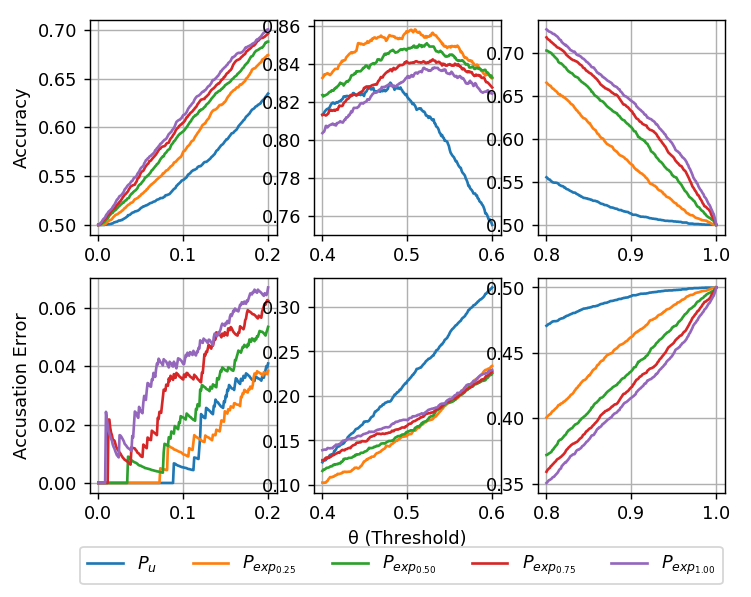
\includegraphics[width=0.7\textwidth]{./pictures/discussion/conv_char_nn_prediction_zoom_50_time.png}
            \caption{Illustrate important intervals for our different
                $P_{exp_\lambda}$ prediction systems for the \gls{conv-char-NN}
                network on the 0.5 split dataset. On the left we have shown the
                beginning of the curves, in the middle we have shown the top
                accuracy and to the right we have shown the end of the curves.}
            \label{fig:conv_char_prediction_zoom_50}
        \end{figure}

        \begin{figure}
            \centering
            \textbf{\glsdesc{conv-char-NN} Prediction System 0.04 Split}\par\medskip
            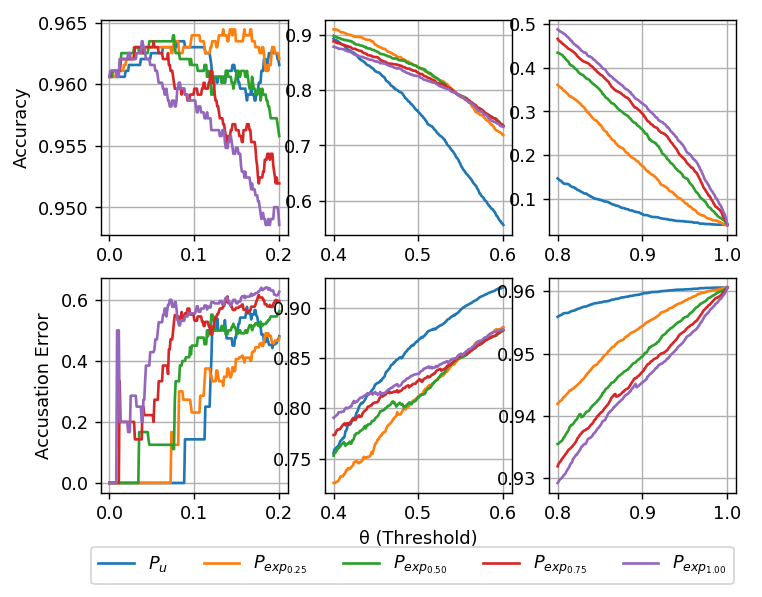
\includegraphics[width=0.7\textwidth]{./pictures/discussion/conv_char_nn_prediction_zoom_04_time.png}
            \caption{Illustrate important intervals for our different
                $P_{exp_\lambda}$ prediction systems for the \gls{conv-char-NN}
                network on the 0.04 split dataset. On the left we have shown the
                beginning of the curves, in the middle we have shown the top
                accuracy and to the right we have shown the end of the curves.}
            \label{fig:conv_char_prediction_zoom_04}
        \end{figure}

        It is hard to say which $\lambda$ produce the best results when looking
        at the Figures. Let us focus on the 0.5 case as that gives a clearer
        picture. For low $\theta$'s we have that $\lambda = 1.0$ gives the
        highest accuracy but with highest accusation error while $\lambda =
        0.25$ gives the lowest accuracy with the lowest accusation error. We see
        a similar picture for high $\theta$'s. There we get the highest accuracy
        but lowest accusation error when $\lambda = 1.0$ and the lowest accuracy
        and highest accusation error when $\lambda = 0.25$. At both extremes we
        have that the highest accuracy is obtained when $\lambda = 1.0$. In the
        middle of the graph however we observe that the highest accuracy AND
        lowest is accusation error is obtained when $\lambda = 0.25$. It seems
        as if the best $\lambda$ value changes depending on what threshold is
        chosen. We will now discuss the three threshold intervals.

        When $\theta \in (0, 0.2)$ higher accuracy is obtained as $\lambda
        \rightarrow 1$ however it is clear that there is diminishing returns
        for increasing $\lambda$. There is a large difference in accuracy
        between $\lambda = 0.25$ and $\lambda = 0.5$, a smaller difference
        between $\lambda = 0.5$ and $\lambda = 0.75$ and an even smaller
        difference between $\lambda = 0.75$ and $\lambda = 1.0$. At the same
        time the accusation error increases as $\lambda \rightarrow 1$ but it
        does not seem that it increases with diminishing returns. The best
        prediction system in this interval is therefore a tradeoff between the
        accusation error and accuracy obtained. You can increase your accuracy
        by increasing $\lambda$ but at the same time the accusation error will
        also rise. We solved that problem by maximizing the accuracy while
        keeping the accusation error under a threshold which seems to have been
        the right thing to do. When looking at the Figure it seems to us as if
        the best weighing for time is either $\lambda = 0.25$ or $\lambda = 0.5$
        as those have low accusation error coupled with fine accuracy. Let us
        consider the reason that the accuracy rises when we give more weight
        to the first assignment. In this interval $\theta$ is low. That means
        that we will get almost all positive cases correct. The accuracy above
        0.5 must consist of those negative cases where the assignment is most
        clearly written by someone else than a candidate author. When we predict
        that negative text against all of a candidate authors texts it has to
        be extremely different for it to get very low scores for all of that
        authors texts. However there is a good chance that it will be different
        from one of the texts i.e. the newest text. Therefore higher $\lambda$
        values has a higher chance of reporting a negative meaning that they
        will obtain a higher accuracy on this part of the graph but also a
        higher accusation error. Similarly lower $\lambda$ values will have a
        lower chance of reporting a negative giving a lower accuracy but also a
        lower accusation error.

        When $\theta \in (0.4, 0.6)$ higher accuracy is obtained as $\lambda
        \rightarrow 0.25$. At the same time the lowest accusation error is also
        obtained when $\lambda$ is low. It is therefore clear that the best
        configuration in this interval is low $\lambda$ values. But it is also
        clear that $\lambda$ should be greater than 0 (not uniform) as the
        uniform weights is clearly worse than all the other. Lets consider why
        that might be the case. Here in the middle of the graph we don't require
        extreme values to produce either negatives or positives. Therefore a
        weigh that is closer to uniform is likely to produce better results
        since it better use information from all texts available.

        When $\theta \in (0.8, 1.0)$ higher accuracy is obtained as $\lambda
        \rightarrow 1.0$. As in the first interval the accuracy is obtained with
        diminishing returns. Unlike the first interval the accusation error is
        now lowest for higher $\lambda$. It is therefore clear that the best
        $\lambda$ value in this interval is $\lambda = 1.0$. Again we have that
        the reason for obtaining greater accuracy when $\lambda$ increases in
        is that at this extreme we will get almost all negative cases correct
        but only a small subset of the positives will be correct. Therefore the
        further away from uniform weights we get we will report more positives
        giving us higher accuracy. In this case however that does not lead
        to higher accusation error since almost all problems is reported as
        negative and the few we move to positive will reduce the accusation
        error. The best $\lambda$ in this case is irrelevant since we would
        never choose a $\theta$ in this range. Such a $\theta$ would lead to way
        to many false accusation.

        This whole discussion has been based on the picture presented
        for the dataset of 50\% positives and 50\% negatives. In Figure
        \ref{fig:conv_char_prediction_zoom_04} we see a slightly different
        picture. When there is less negatives available $\lambda = 1.0$ does
        not lead to the best results in the interval $\theta \in (0, 0.2)$.
        Instead $\lambda = 0.25$ or $\lambda = 0.5$ seem to give the best
        results. Since it is now more risky to report a negative it makes sense
        that weights closer to uniform performs better since more is required
        to make them report a negative in this interval. It is still clear that
        $P_\mathcal{U}$ is the worst prediction system so we can still conclude
        that the newest assignment is more indicative of writing style than the
        oldest.

        To get a better idea of weighing based on time we created looped through
        the authors in the test set D. We created a positive sample for each
        of the authors and used \gls{conv-char-NN} to predict each of the
        authors texts. We then computed the average score of the newest text,
        the average score of the second newest text, and so on. If the students
        writing style changes over time we would expect higher scores in the
        beginning and lower scores at the end. The output of the experiment
        resulted in,

        \begin{equation}
            (0.78884, 0.76248, 0.74841, 0.70693, 0.69037, 0.66954, 0.65441,
            0.64049, 0.62651, 0.61295, \dots)^T
        \end{equation}

        where the average score of the newest text is shown first and the
        average score of the oldest text last. That vector clearly shows that
        writing style changes over time and it is therefore a good idea to use
        some sort of time based prediction system.

    \item[$P_l$]

        The idea behind the length based prediction system was that longer
        texts would better reflect the writing style of an author. Some
        of the texts in the dataset are only a few hundred characters
        long which means that only few of the n-grams the networks
        are looking for will be present in those texts. In Figure
        \ref{fig:conv_char_prediction_zoom_50_text_length} we have shown a
        comparison between $P_\mathcal{U}$ and $P_l$. It can be seen there that
        it is always better to weight based on text length than it is to just
        use uniform weights. The curves follow each other closely but $P_l$
        have slightly higher accuracy and slightly lower accusation error than
        $P_\mathcal{U}$.

        \begin{figure}
            \centering
            \textbf{\glsdesc{conv-char-NN} Prediction System 0.04 Split}\par\medskip
            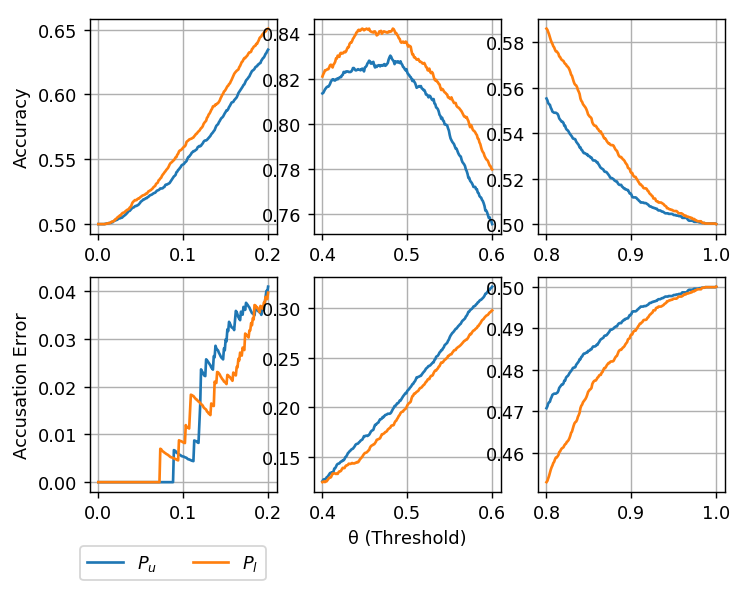
\includegraphics[width=0.7\textwidth]{./pictures/discussion/conv_char_nn_prediction_zoom_50_text_length.png}
            \caption{Illustrate important intervals for our $P_l$ prediction
                systems for the \gls{conv-char-NN} network on the 0.5 split
                dataset. On the left we have shown the beginning of the curves,
                in the middle we have shown the top accuracy and to the right we
                have shown the end of the curves.}
            \label{fig:conv_char_prediction_zoom_50_text_length}
        \end{figure}

        That is exactly the result we expected and shows that it was a good idea
        to look at text length as part of our prediction systems. We have not
        shown the results of the 0.04 split as the same is the case there.

    \item[$P_{lepx_{0.25}}$]

        This prediction system were a combination of the time based and text
        length based prediction systems. Multiple different networks had this
        configuration as the configuration that maximized accuracy. We have
        already concluded that both $P_l$ and $P_{exp_\lambda}$ was better
        weightings than $P_\mathcal{U}$. So the interesting thing about this
        weight is not whether or not it beats $P_\mathcal{U}$, but rather
        whether or not it is better than $P_l$ and $P_{exp_\lambda}$. In Figure
        \ref{fig:conv_char_prediction_zoom_50_time_and_length} we have shown the
        performance of $P_{lexp_\lambda}$.

        \begin{figure}
            \centering
            \textbf{\glsdesc{conv-char-NN} Prediction System 0.04 Split}\par\medskip
            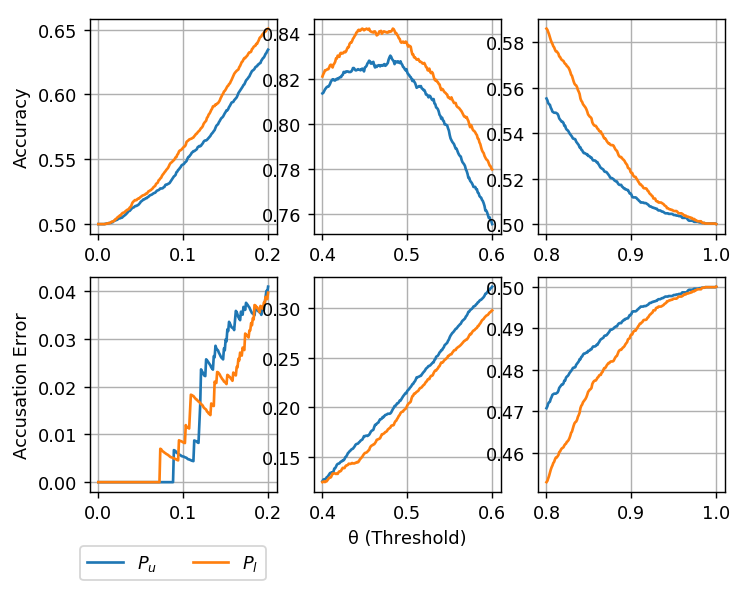
\includegraphics[width=0.7\textwidth]{./pictures/discussion/conv_char_nn_prediction_zoom_50_text_length.png}
            \caption{Illustrate important intervals for our $P_l$ prediction
                systems for the \gls{conv-char-NN} network on the 0.5 split
                dataset. On the left we have shown the beginning of the curves,
                in the middle we have shown the top accuracy and to the right we
                have shown the end of the curves.}
            \label{fig:conv_char_prediction_zoom_50_text_length}
        \end{figure}

        In that Figure we see that $P_{exp_{0.25}}$ has generally better
        performance than $P_{lexp_{0.25}}$ except right at the maximum accuracy.
        At the maximum accuracy $P_{lexp_{0.25}}$ is able to just barely beat
        $P_{exp_{0.25}}$. Almost all the networks used the $P_{lexp_{0.25}}$
        prediction system as the best prediction system and it must be this
        small difference that causes that.

        It is interesting that the performance of $P_{lexp_{0.25}}$ is only best
        right at the maximum accuracy. Maybe that is due to something similar to
        the effect we saw with $P_{exp_{\lambda}}$ where higher $\lambda$ values
        was best at the extremes and lower $\lambda$ values were better in the
        middle of the graphs.

\end{description}


\begin{figure}
    \centering
    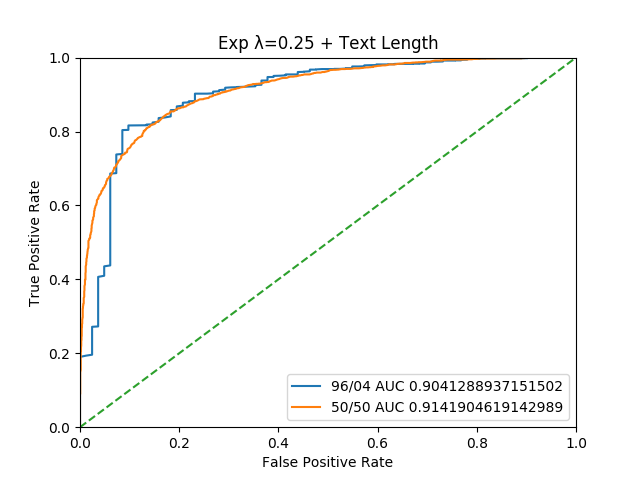
\includegraphics[width=\textwidth]{./pictures/discussion/ROC_Network6.png}
    \caption{\gls{ROC} Curve, and AUROC for \gls{conv-char-word-NN}}
\end{figure}

\begin{figure}
    \centering
    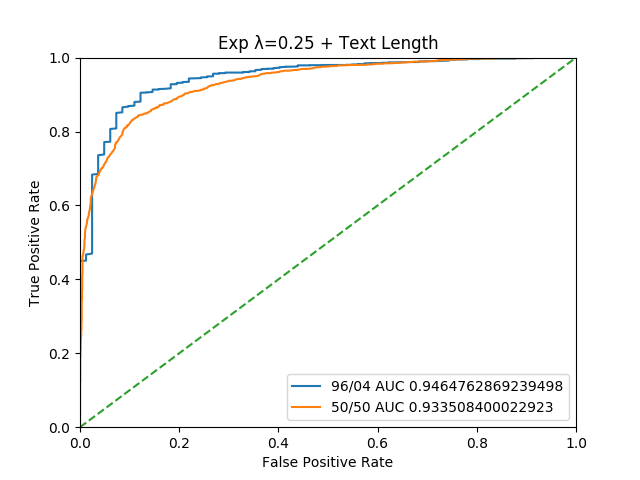
\includegraphics[width=\textwidth]{./pictures/discussion/ROC_Network3.png}
    \caption{\gls{ROC} Curve, and AUROC for \gls{conv-char-NN}}
\end{figure}

\begin{figure}
    \centering
    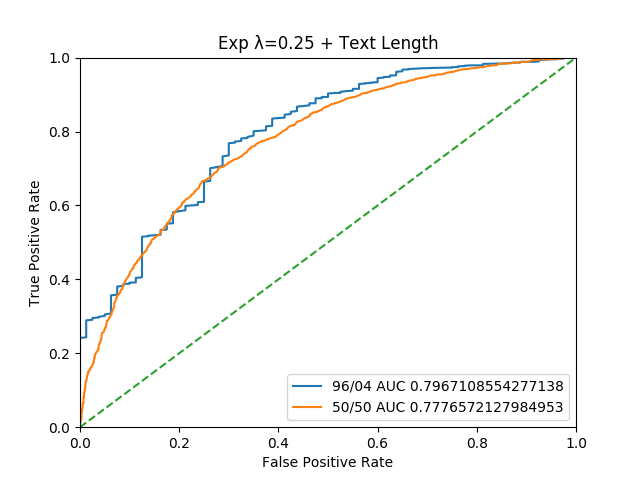
\includegraphics[width=\textwidth]{./pictures/discussion/ROC_RNN.png}
    \caption{\gls{ROC} Curve, and AUROC for \gls{rec-sent-NN}}
\end{figure}
